\documentclass{article}
%-------------------------------------------------------
\usepackage{graphicx}
\usepackage{subcaption}
\usepackage{amsmath}
%-------------------------------------------------------
\begin{document}
%-------------------------------------------------------
\title{EV On-Board Charger : Power Factor Correction}
\author{Mohamed Gueni}
\date{\today}
%-------------------------------------------------------
\maketitle
%-------------------------------------------------------
\tableofcontents
\section{Block Diagram}

The block diagram of the PFC design is shown in Figure \ref{fig:PFC}. The PFC takes input from the Electric Vehicle Supply Equipment (EVSE) which later could be the mains plug (1ph ).
The PFC stage performs power factor correction and boosts the voltage to a specific high DC voltage before delivering DC power to the DC-link at the output.

%-------------------------------------------------------
\begin{figure}[htbp]
    \centering
    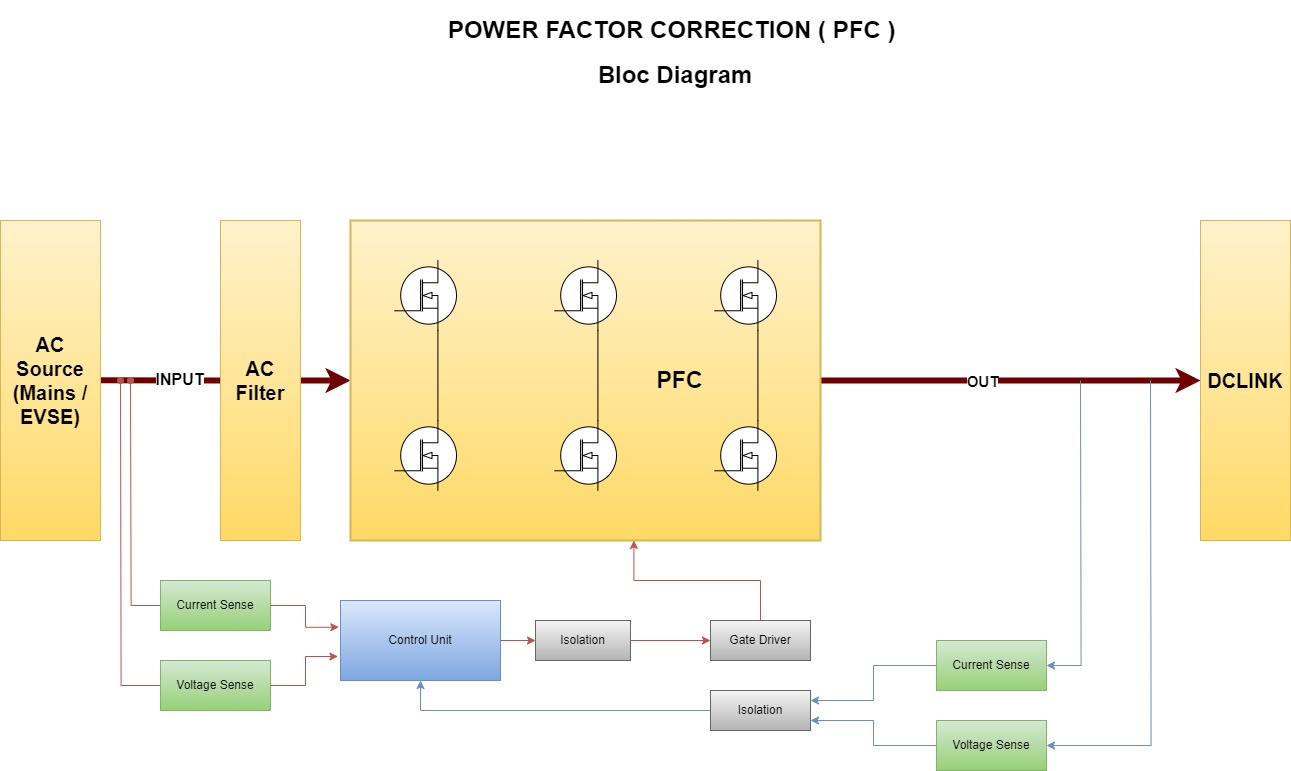
\includegraphics[width=\textwidth]{PFC.jpg}
    \caption{PFC Block Diagram}
    \label{fig:PFC}
\end{figure}
%-------------------------------------------------------
The DC Link at the output of the PFC would carry out the DC input power to the cascaded LLC bloc(s) which will be studied later on.
%-------------------------------------------------------
\section{Block Description}
In this document we will go through all sections of the power factor correction bloc starting with a brief description of the input power source which is an external part to this project and will only be included for simulation purposes.Then we will dive into the topology selected for this PFC stage and the switches technology and references which we'll start with.
Note that later in the simulation phase we would conduct a couple of efficiency simulations between multiple switches from different suppliers in order to determine the one with the most efficiency and less switching and conduction losses in this design.
%-------------------------------------------------------
\subsection{EVSE Input}
The EVSE (Electric Vehicle Supply Equipment) provides the input power to
the on-board charger. It supplies AC or DC (bypass the OBC functions) power from the external power source.in this project we only interested in modeling the input source in simulation phases such as inside Plecs models.
%-------------------------------------------------------
\subsection{AC Filter}
The first stage of the OBC is the EMI filter. During this stage AC power is filtered to remove any undesirable noise from the typical AC sine wave that is expected. 
At the input of our system, the input can present some imperfections due to the high switching components involved in the following stages.Radiated EMI from other components can also be picked up on power cabling, adding to conducted levels. The system can experience at its input mainly two types of Electromagnetic interference (EMI) which are Differential Mode (DM) and Common Mode (CM) Noise.(Figure \ref{fig:ac_filter})
%-------------------------------------------------------
\begin{figure}[htbp]
    \centering
    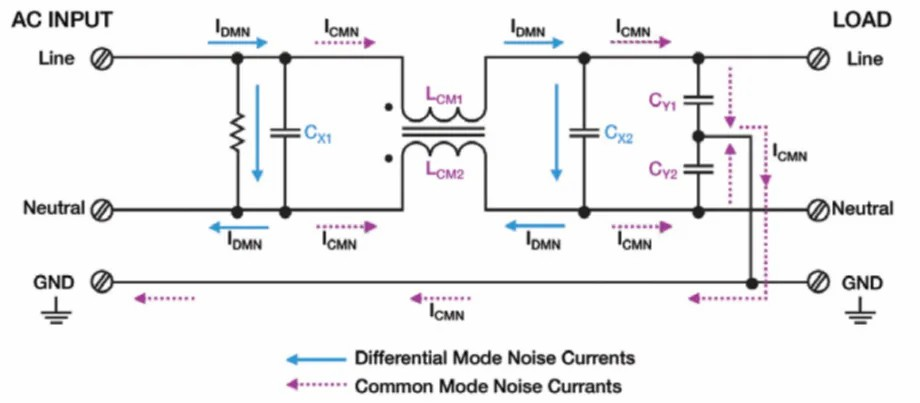
\includegraphics[width=\textwidth]{ac_filter.jpg}
    \caption{AC filter noise path.}
    \label{fig:ac_filter}
\end{figure}
%-------------------------------------------------------

DM noise is conducted on the line and neutral, in opposite directions. The basic DM filter uses a single-winding inductor inserted into the line path, along with a capacitor from line to neutral, thus blocking noise from propagating through the system.

CM noise is noise conducted on both the line and neutral (ground) but in the same direction. The basic CM filter uses a dual-winding inductor in both line and neutral paths, plus a capacitor from line to ground.
%-------------------------------------------------------
\begin{figure}[htbp]
    \centering
    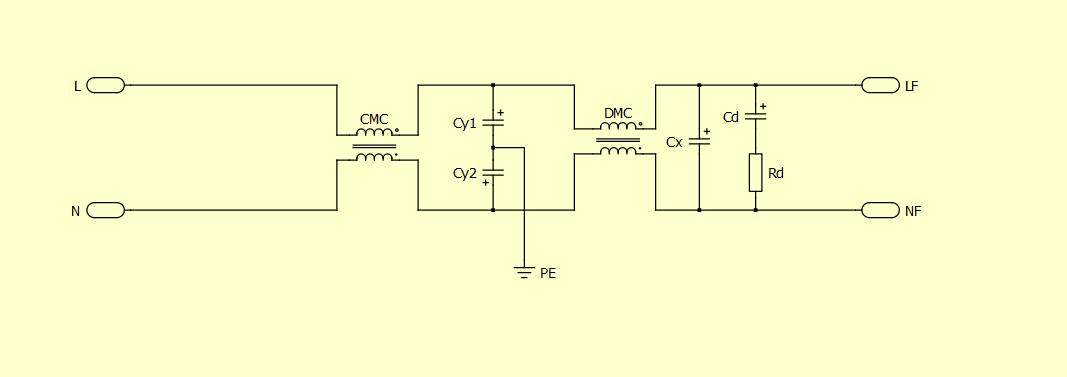
\includegraphics[width=\textwidth]{modular_EMI Plecs model.png}
    \caption{filter Plecs model.}
    \label{fig:modular_EMI_Plecs_model}
\end{figure}
%-------------------------------------------------------
As presented in Figure \ref{fig:modular_EMI_Plecs_model} , a typical but basic EMI filter uses the CX capacitors to attenuate differential mode noise, and an inductor-capacitor combination to reduce common mode noise.

%-------------------------------------------------------
Designing an AC EMI (Electromagnetic Interference) filter for an onboard charger involves several stages to reduce conducted and radiated emissions.the EMI filter limits voltage and current spikes that can be harmful.Most commonly these filters are made up of X and Y Safety Capacitors, Common Mode Chokes and AC Harmonic Filter Capacitors.   
%-------------------------------------------------------
\subsubsection{Common Mode (CM) Filter:}
Purpose:
Attenuate common mode noise, which flows in the same direction on all three phases and the neutral.
Components:
Common mode choke
Common mode capacitors

%-------------------------------------------------------
\subsubsection{Differential Mode (DM) Filter:}
Purpose:
Attenuate differential mode noise, which flows in opposite directions on different phases.
Components:
Differential mode choke
Differential mode capacitors

%-------------------------------------------------------

Note that this could be an unfinished design and we could end up simplifying it further by selecting a choke for the common mode with a certain leakage inductance which we could use as the main inductance for the differential mode filtering.
we could also add a fuse at the input and an x capacitor.
%-------------------------------------------------------

\begin{figure}[htbp]
    \centering
    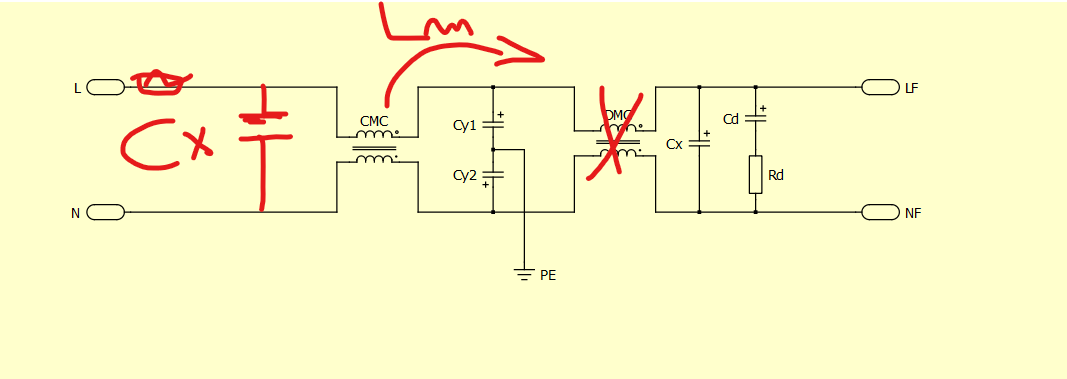
\includegraphics[width=\textwidth]{Filter plecs model simplification.png}
    \caption{filter Plecs model.}
    \label{fig:Filter plecs model simplification.}
\end{figure}
%-------------------------------------------------------
\subsubsection{CISPR 25:}
CISPR 25 provides specific limits and requirements for conducted and radiated emissions in various frequency bands. Here are some typical values and ranges specified by CISPR 25 for automotive applications:

Conducted Emissions:
Frequency Range: Typically from 150 kHz to 108 MHz.
Conducted Emissions Limits: Vary depending on the frequency band and the class of the vehicle (e.g., passenger car, commercial vehicle).
For example, the limit for passenger cars might be around 40 dBµV in the frequency range of 150 kHz to 22 MHz.
For commercial vehicles, the limit might be higher, around 60 dBµV in the same frequency range.

Radiated Emissions:
Frequency Range: Typically from 30 MHz to 1 GHz.
Radiated Emissions Limits: Given in terms of field strength, often measured in dBµV/m at various distances from the vehicle.
For example, at a distance of 10 meters, the limit might be around 30 dBµV/m in the frequency range of 30 MHz to 1000 MHz.

%-------------------------------------------------------
\subsubsection{Values and Calculations:}
Aside from considering the standard CISPR 25 for determining values of filter components generally. We also going to consider professor Middlebrook stability criteria and input filter interaction to start with.


%-------------------------------------------------------
\begin{figure}[htbp]
    \centering
    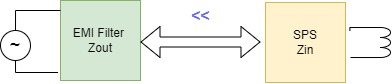
\includegraphics[width=\textwidth]{Middlebrook stability criteria.jpg}
    \caption{Middlebrook stability criteria.}
    \label{fig:Middlebrook stability criteria.}
\end{figure}
Middlebrook stability criteria and input filter interaction states in general  ""  if the input impedance of a converter, Zin, is always greater than the output impedance of the filter, Zout, \[ Z_{\text{in(PFC)}} >> Z_{\text{out(Filter)}} \] then a stable power supply will remain stable when the filter is connected. "".
We could either measure the input impedance of the PFC (the SPS in our case) or like in this case we are interested in making a first approximation where : 
\[
Z_{\text{in}} =  \frac{V_{\text{in}}^2\times\eta}{P_{\text{out}}}
\]

\begin{align*}
\text{where:} \\
 V_{\text{in}} &\text{ is the input voltage (V)} \\
\eta &\text{ is the efficiency ( ) } \\
 P_{\text{out}} &\text{ is the output power (W}\text{)}
\end{align*}

and the output impedance of the EMI input filter is :

\[
Z_{\text{out}} =  \sqrt(\frac{L}{C})
\]

\begin{align*}
\text{where:} \\
 L &\text{ is the inductance value (H)} \\
 C &\text{ is the capacitor value (F}\text{)}
\end{align*}
We determine the cutoff frequency of the filter by :

\[
fc_{\text{filter}} =  \frac{1}{2\times\pi\times\sqrt{L\times C}}
\]

\begin{align*}
\text{where:} \\
 L &\text{ is the inductance value (H)} \\
 C &\text{ is the capacitor value (F}\text{)}
\end{align*}
In general we are interested in attenuating the frequencies higher than the maximum switching frequency of the PFC (70KHz) so as a rule of thumb we start by considering the cutoff frequency of the filter as :

\[
fc_{\text{filter}} =  75 KHz
\]

The process moving forward will be about a mixture between using mathematical formulas , trial and error , simulation and logic related to multiple aspects to name a few : physical size of the components and other characteristics and the availability of certain values of components in the market (good luck finding certain values if they ever existed ).

First we could Find the approximated Input impedance of the system in series with the input filter using professor Middlebrook's approximation:

\[
Z_{\text{in}} =  
\]

which then means that in order for the system to not get affected by the addition of the filter : 
\[Z_{\text{out(Filter)}} << \]

Given we already know Zout filter is dependent on the L and C values at its output. We could select one of the values (choose the most commonly used / tested values) and use a reactance paper and simulation software such as Plecs and LtSpice to narrow down a small margin of values for both C and L and simulate all range.





%-------------------------------------------------------
%-------------------------------------------------------
%-------------------------------------------------------
%-------------------------------------------------------
\section{References}

\begin{enumerate}
    
    \item R. W. Erickson, \textit{Fundamentals of power electronics}, New York: Chapman \& Hall, 1997.
    \item S. Ahmed, “Controlled on-time power factor correction circuit with input filter”, M.Sc. thesis, Virginia Polytechnic Institute and State University, Blacksburg, VA, 1990.
    \item V. Vlatkovic, D. Borojevic, F. C. Lee, “Input filter design for power factor correction circuits”, \textit{IEEE Transactions on Power Electronics}, vol. 11, no. 1, pp. 199-205, Jan. 1996.
    \item J. S. Glaser, A. F. Witulski, “Design issues for high power factor AC-DC converters systems”, in \textit{IEEE Power Electronics Specialists Conference 1995 Record}, pp. 542-548.
    \item Y. Jang, R. W. Erickson, “Physical origins of input filter oscillations in current programmed converters”, \textit{IEEE Transactions on Power Electronics}, vol. 7, no. 4, pp. 725-733, Oct. 1992.
    \item R. B. Ridley, “Average small signal analysis of the Boost Power Factor Correction Circuit”, in \textit{Virginia Power Electronics Center Seminar Proceedings 1989}.
\end{enumerate}
%-------------------------------------------------------
\section{Units}

\begin{enumerate}
    \item Farads (\textbf{F}).................: Unit of capacitance.
    \item Amps (\textbf{A})..................: Unit of electric current.
    \item Volts (\textbf{V})...................: Unit of electric potential.
    \item Ohms (\textbf{$\Omega$})...................: Unit of electrical resistance.
    \item Henrys (\textbf{H}).................: Unit of inductance.
    \item Watts (\textbf{W}).................: Unit of power.
    \item Hertz (\textbf{Hz}).................: Unit of frequency.
    \item Teslas (\textbf{T})...................: Unit of magnetic flux density.
    \item Webers (\textbf{Wb}).............: Unit of magnetic flux.
    \item Decibels (\textbf{dB}).............: Unit of measurement for the power level of an electrical signal.(or the intensity of a sound )
\end{enumerate}
%-------------------------------------------------------
\end{document}
%-------------------------------------------------------